
\subsection{Monte Carlo approximation of the VR bound}
\label{sec:chap4_vrbound_sampling}

Although we have seen some nice properties of the VR bound optimisation through the mean-field approximation example, we also note that when $\alpha \neq 1$, the VR bound is usually just as intractable as the marginal likelihood for many other useful models. Also Theorem \ref{thm:chap4_vrbound_alpha_vi} suggests that the VR bound is to be minimised when $\alpha < 0$, which performs disastrously in MLE context.
%
 As we shall see, these issues are addressed by the MC approximation that we will be developing as follows, under certain conditions. Therefore, MC-VR can be applied to precisely the same set of models as MC-VI \citep{paisley:bbvi2012, salimans:reparam2013, ranganath:bbvi2014, kucukelbir:advi2015}.

Consider learning a latent variable model with MLE as a running example, where the model is specified by a conditional distribution $p(\bm{x}|\z, \bm{\varphi})$ and a prior $p(\z| \bm{\varphi})$ on the latent variable $\z$. Examples include latent variable models treated by the variational auto-encoder (VAE) approach \citep{kingma:vae2014, rezende:vae2014} that parametrises the likelihood with a (deep) neural network. MLE requires $\log p(\bm{x})$ which is obtained by marginalising out $\z$ and is often intractable, so the VR bound is considered as an alternative optimisation objective. However instead of using exact bounds, a simple Monte Carlo (MC) method is deployed, which uses a finite number of samples $\z_k \sim q(\z|\bm{x}), k = 1, ..., K$ to approximate the VR bound $\mathcal{L}_{\alpha} \approx \hat{\mathcal{L}}_{\alpha, K}$:
\begin{equation}
\label{eq:sampling_estimate}
\hat{\mathcal{L}}_{\alpha, K}(q; \bm{x}) = \frac{1}{1 - \alpha} \log \frac{1}{K} \sum_{k=1}^K \left[\left( \frac{p(\z_k, \bm{x})}{q(\z_k|\bm{x})} \right)^{1 - \alpha} \right].
\end{equation}
The importance weighted auto-encoder (IWAE) \citep{burda:iwae2016} is a special case of this framework with $\alpha = 0$ and $K < +\infty$. But unlike traditional VI, here the MC approximation is biased. Fortunately we can characterise the bias by the following theorems (proofs provided in Appendix \ref{sec:appendix_proof_chap4}).
%
%
%%%%% theorem %%%%%
\begin{theorem}
\label{thm:chap4_vrbound_sampling_bound}
Assume $\mathbb{E}_{\{\z_k\}_{k=1}^K} [ |\hat{\mathcal{L}}_{\alpha, K}(q; \bm{x})| ] < + \infty$ and $|\mathcal{L}_{\alpha}| < +\infty$. Then $\mathbb{E}_{\{\z_k\}_{k=1}^K} [ \hat{\mathcal{L}}_{\alpha, K}(q; \bm{x}) ]$ as a function of $\alpha \in \mathbb{R}$ and $K \geq 1$ is: \\
1) \textbf{non-decreasing} in $K$ for fixed $\alpha \leq 1$, and \textbf{non-increasing} in $K$ for fixed $\alpha \geq 1$; \\
2) $\mathbb{E}_{\{\z_k\}_{k=1}^K} [ \hat{\mathcal{L}}_{\alpha, K}(q; \bm{x}) ] \rightarrow \mathcal{L}_{\alpha}$ as $K \rightarrow +\infty$; \\
3) \textbf{continuous} and \textbf{non-increasing} in $\alpha$ with fixed $K$.
\end{theorem}

%%%%%% corollary %%%%%
\begin{corollary}
\label{thm:chap4_vrbound_alpha_k_existence}
For finite $K$, either $\mathbb{E}_{\{\z_k\}_{k=1}^K} [ \hat{\mathcal{L}}_{\alpha, K}(q; \bm{x}) ] < \log p(\bm{x})$ for all $\alpha$, or there exists $\alpha_K \leq 0$ such that $\mathbb{E}_{\{\z_k\}_{k=1}^K} [ \hat{\mathcal{L}}_{\alpha_K, K}(q; \bm{x}) ] = \log p(\bm{x})$ and $\mathbb{E}_{\{\z_k\}_{k=1}^K} [ \hat{\mathcal{L}}_{\alpha, K}(q; \bm{x}) ] > \log p(\bm{x})$ for all $\alpha < \alpha_K$. Also $\alpha_K$ is \textbf{non-decreasing} in $K$ if exists, with $\lim_{K \rightarrow 1} \alpha_K = -\infty$ and $\lim_{K \rightarrow +\infty} \alpha_K = 0$.
\end{corollary}
%%%%%%%%%%%%%%%%

%
The intuition behind the theorems is visualised in Figure \ref{fig:chap4_vrbound_divergence_sampling}. By definition, the exact VR bound is a lower-bound or upper-bound of $\log p(\bm{x})$ when $\alpha > 0$ or $\alpha < 0$, respectively. However the MC approximation $\mathbb{E}[\hat{\mathcal{L}}_{\alpha, K}]$ biases the estimate towards $\mathcal{L}_{\text{VI}}$, where the MC approximation of the bound can be improved using more samples. Thus for finite samples and under mild conditions, negative alpha values can potentially be used to improve the accuracy of the approximation, although the MC approximation for these alpha values is no longer guaranteed to be an upper bound.
%
Figure \ref{fig:chap4_vrbound_divergence_simulation} shows an empirical evaluation by computing the exact and the MC approximation of the R{\'e}nyi divergence. In this example $p$, $q$ are 2-D Gaussian distributions with $\bm{\mu}_p = [0, 0]$, $\bm{\mu}_q = [1, 1]$ and $\bm{\Sigma}_p = \bm{\Sigma}_q = \bm{I}$. The sampling procedure is repeated 200 times to estimate the expectation. Clearly for $K = 1$ it is equivalent to an unbiased estimate of the KL-divergence for all $\alpha$ (even though now the estimation is biased for $\mathrm{D}_{\alpha}^{R}$). For $K > 1$ and $\alpha < 1$, the MC method under-estimates the VR bound, and the bias decreases with increasing $K$. For $\alpha > 1$ the inequality is reversed also as predicted.


\begin{figure*}[t]
 \centering
 \subfigure[MC approximated VR bounds.]{
 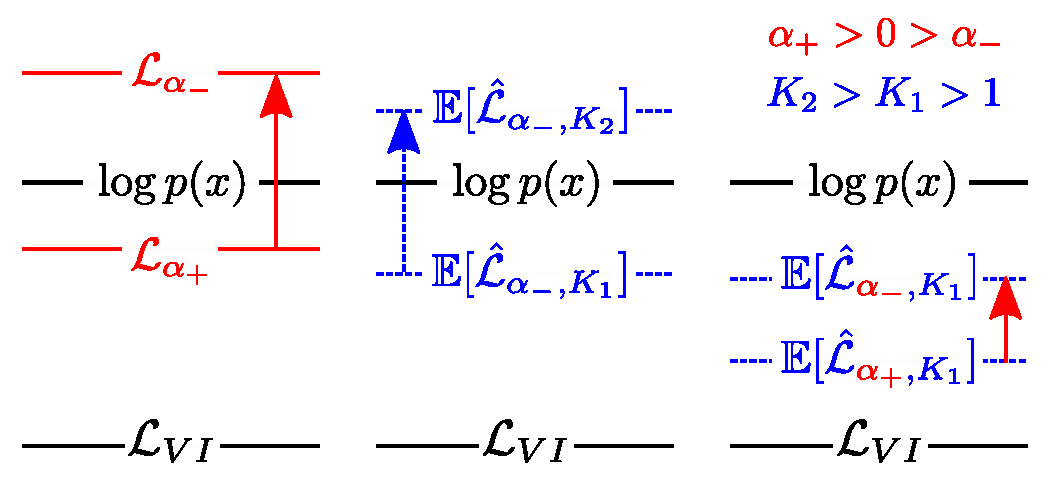
\includegraphics[width=0.6\linewidth]{sampling_bound_full.pdf}
 \label{fig:chap4_vrbound_divergence_sampling}}
 \hspace{0.1in}
 \subfigure[Simulated MC approximations.]{
 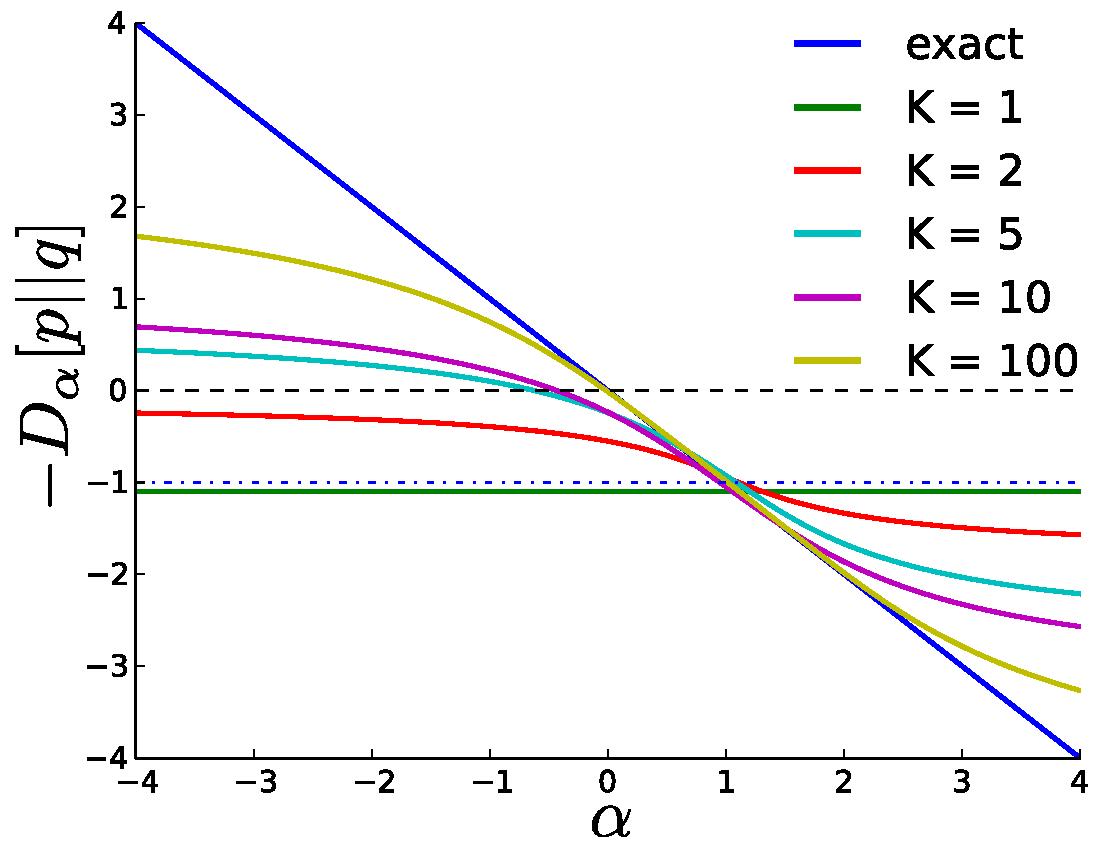
\includegraphics[width=0.34\linewidth]{divergence_sampling.pdf}
 \label{fig:chap4_vrbound_divergence_simulation}}
 \vspace{-0.1in}
 \caption{(a) An illustration for the bounding properties of MC approximations to the VR bounds (non-increasing in $\alpha$ and non-decreasing in $K$ when $\alpha \leq 1$). (b) The bias of the MC approximation, where the dash-dotted line on top of the green line ($K=1$) is the analytical value of $-\mathrm{KL}[p||q]$. Best viewed in colour and see the main text for details.}
\end{figure*}